% CMC/TSP submission manuscript, v71 claim-calibrated language revision.
\documentclass[cmc,article,submit,moreauthors,pdftex]{Definitions/tsp}
\input{Definitions/package}
\input{Definitions/unicode}
\usepackage[OT1,OT2,T2A,T2B,T2C,T3,T5,T1]{fontenc}
\usepackage[russian,english]{babel}
\usepackage{booktabs}
\usepackage{tabularx}
\usepackage{float}
\usepackage{enumitem}
\usepackage{amsmath,amssymb}
\usepackage{array}
\usepackage{needspace}
\usepackage{longtable}
\setlength{\headheight}{38.3pt}
\setlength{\floatsep}{8pt plus 2pt minus 2pt}
\setlength{\textfloatsep}{10pt plus 2pt minus 3pt}
\setlength{\intextsep}{9pt plus 2pt minus 2pt}
\makeatletter
\setlength{\@fptop}{0pt}
\setlength{\@fpsep}{10pt}
\setlength{\@fpbot}{0pt plus 1fil}
\makeatother
\renewcommand{\topfraction}{0.95}
\renewcommand{\bottomfraction}{0.90}
\renewcommand{\textfraction}{0.06}
\renewcommand{\floatpagefraction}{0.75}
\newcolumntype{Y}{>{\centering\arraybackslash}X}
\newcolumntype{Z}{>{\raggedright\arraybackslash}X}
\newcommand{\tabnote}[1]{\par\smallskip\noindent\begin{minipage}{\linewidth}\footnotesize\emph{Note}: #1\end{minipage}\par}
\graphicspath{{Figures/}}

\continuouspages{}
\firstpage{1}
\makeatletter
\setcounter{page}{\@firstpage}
\makeatother
\pubvolume{0}
\issuenum{0}
\elocationid{0}
\articlenumber{0}
\pubyear{2026}
\copyrightyear{2026}
\datereceived{Day Month Year}
\dateaccepted{Day Month Year}
\dateonlinefirst{}
\datepublished{Day Month Year}

\Title{Energy-Gated DA-TPP: Batch Active Learning for Early Target Recovery in Generated Crystal Pools}
\newcommand{\orcidauthorE}{0009-0003-3796-4444}
\Author{Yueyang Zhang\textsuperscript{1,\#}, Jinxuan Liu\textsuperscript{1,\#}, Tianyu Li\textsuperscript{2}, Xiangxiru Xiong\textsuperscript{3}, Yingjie Zhang\orcidE{}\textsuperscript{2,*} and Baohua Tan\textsuperscript{4,5,6,*}}
\AuthorCitation{Zhang Y, Liu J, Li T, Xiong X, Zhang Y, Tan B}
\AuthorNames{Yueyang Zhang, Jinxuan Liu, Tianyu Li, Xiangxiru Xiong, Yingjie Zhang and Baohua Tan}
\address{%
\textsuperscript{1}Hubei University of Technology, No. 28 Nanli Road, Hongshan District, Wuhan, Hubei 430068, China

\textsuperscript{2}Department of Applied Physics, The Hong Kong Polytechnic University, Hung Hom, Kowloon, Hong Kong, China

\textsuperscript{3}Department of Mathematics and Information Technology, The Education University of Hong Kong, 10 Lo Ping Road, Tai Po, New Territories, Hong Kong, China

\textsuperscript{4}School of Science (School of Chip Industry), Hubei University of Technology, Wuhan, 430068, China

\textsuperscript{5}National ``111 Research Center'' Microelectronics and Integrated Circuits, Hubei University of Technology, Wuhan, 430068, China

\textsuperscript{6}Department of Architecture and Built Environment, Faculty of Engineering, University of Nottingham, Nottingham, NG7 2RD, United Kingdom

\textit{E-mail addresses:} 2411631131@hbut.edu.cn (Y. Zhang); 2511611209@hbut.edu.cn (J. Liu); tianyu.li@connect.polyu.hk (T. Li); s1165476@s.eduhk.hk (X. Xiong); yingjieyj.zhang@connect.polyu.hk (Y. Zhang); tbh@hbut.edu.cn (B. Tan)
}
\corres{Corresponding Authors: Yingjie Zhang. Email: yingjieyj.zhang@connect.polyu.hk; Baohua Tan. Email: tbh@hbut.edu.cn}
\firstnote{These authors contributed equally to this work.}

\abstract{Generated crystal pools often exceed the computational budgets
available for first-principles validation, making effective early-stage
prioritization essential. Exploitation-based acquisition efficiently identifies
candidates with high predicted target probabilities, while batch-level chemical
structure offers additional information for improving screening efficiency. We
introduce Energy-Gated Diversity-Aware Target Probability Prioritization
(Energy-Gated DA-TPP), an adaptive batch active-learning framework that
integrates target probability, predictive uncertainty, representation-space
diversity, and chemical-group coverage through energy-gated selection. Starting
from a Predicted-Target Greedy batch, Gate evaluates score separation and group
concentration, retaining well-resolved batches and activating diversity-aware
reconstruction when diagnostic thresholds indicate redundancy. This design
allocates diversity according to the evolving structure of the candidate front
and improves the balance between target exploitation and batch coverage.
Energy-Gated DA-TPP was evaluated on a MatterGen-derived Li--M--O spinel-like
pool containing 640 candidates and 78 targets defined by a fixed ALIGNN
formation-energy interval. Within the first 80 queries, Gate recovered 26
targets compared with 19 for Greedy, a 36.8\% increase in early target recovery.
The normalized area under the target-recovery curve through 160 queries
increased from 0.2795 to 0.3205, while both policies recovered all 78 targets by
320 queries. Ablation results linked the early-budget reordering primarily to
group-triggered batch repair. An acquisition-blind DFT-evaluability model based
on composition, structure, and CHGNet/MACE-MP descriptors achieved a nested
leave-one-out ROC--AUC of 0.820 and estimated 16.63 evaluable targets for Gate
versus 10.99 for Greedy at 80 queries. Four generated LiCr$_2$O$_4$ candidates
also completed the prescribed PAW--PBE+$U$ relaxation--static workflow. These
results show that adaptive gating can concentrate diversity correction on
redundancy-prone batches, accelerating early target recovery while preserving
final recall. Energy-Gated DA-TPP provides an efficient and auditable strategy
for finite-budget screening of large generated-material pools.}
\keyword{Active learning; generated crystals; batch acquisition; target recovery; conditional diversity; DFT feasibility}

\begin{document}
% Main body, v71 claim-calibrated language revision.
\section{Introduction}

Crystal generators can now produce more plausible structures than a routine
first-principles campaign can examine
\cite{ref-cdvae,ref-diffcsp,ref-mattergen,ref-chemeleon}. This shifts an
important decision to the period immediately after generation. Candidates must
be ordered before their electronic-structure behaviour is known. A learned
property can guide that order, but it cannot show that a later calculation will
converge or that the structure will be stable against competing phases.

Here, the generated candidate pool is the fixed list presented to the selector. A
surrogate target is a candidate whose precomputed ALIGNN label falls in the chosen
interval. DFT evaluability instead concerns completion and reconstructability
of a specified calculation chain. Thermodynamic stability requires a separate
phase comparison. CGCNN determines the query order, whereas ALIGNN supplies the
reference labels used to assess it \cite{ref-cgcnn,ref-alignn}. Published CHGNet
and MACE-MP models are applied only after selection to create lower-fidelity
structural and energetic records \cite{ref-chgnet,ref-macemp}.

Each acquisition round contains 16 candidates. Because the entire batch
is chosen before the next labels arrive, a high-scoring front can devote much
of a round to one coarse chemical group. Such concentration may reflect
redundancy, but it may also be justified when that group is rich in targets.
Applying a diversity penalty to every round therefore has a cost as well as a
possible benefit.

Energy-Gated Diversity-Aware Target Probability Prioritization (Energy-Gated
DA-TPP) addresses this choice by testing the Greedy front before changing it.
The direct top-$b$ list is retained when its score separation and group balance
pass the gate. Otherwise, a replacement score combines target probability,
predictive spread, representation distance, and a repeated-group penalty.

The primary objective is to test whether Gate improves normalized AUTC through
160 queries relative to Predicted-Target Greedy under independently initialized
held-out seeds. Secondary analyses examine checkpoint recovery, route ablations,
the Mn-oxide fallback, post-selection DFT evaluability, MLIP calibration, and four
LiCr$_2$O$_4$ workflows. These analyses retain separate evidence levels for
surrogate-target ordering and later screening stages.

\section{Related Work}

Large repositories such as the Materials Project, OQMD, AFLOW, and JARVIS
supply much of the structured data used by supervised materials screening
\cite{ref-materials-project,ref-oqmd,ref-aflow,ref-jarvis}. A generated pool is
less mature. It may contain close structural variants and labels whose energy
convention differs from a later DFT calculation. These issues have become more
visible as diffusion and variational models produce candidate structures at
scale \cite{ref-cdvae,ref-diffcsp,ref-mattergen,ref-chemeleon}.

Pool-based active learning assigns the next part of a finite label budget. For
interval recovery, direct target-probability ranking is the exploitation
baseline. BADGE, core-set selection, KMeans++ seeding, and local penalization
reduce batch redundancy through gradients, coverage, or distance
\cite{ref-badge,ref-coreset,ref-kmeanspp,ref-localpenalization}. They introduce
diversity directly. Energy-Gated DA-TPP first constructs the exploitation batch
and changes it only when the current front fails its diagnostics.

A target-recovery curve says nothing about completion of a prescribed DFT
workflow. We therefore treat DFT evaluability as a separate post-selection
metric. Pretrained interatomic potentials add another
low-cost layer by returning energies, forces, stresses, and relaxed geometries
for a large pool \cite{ref-chgnet,ref-macemp}. Here their outputs form the
low-fidelity record and support a small comparison with reconstructable DFT
energies. Neither the evaluator nor the MLIPs can alter the archived query order.

\section{Problem Formulation}

Consider a finite pool $\mathcal{C}=\{c_i\}_{i=1}^{N}$. Its frozen reference
table contains an oracle label $y_i$ for each candidate, but the acquisition
loop receives $y_i$ only after candidate $i$ is queried. Given bounds $L$ and
$U$, the indicator $z_i=\mathbb{I}(L\leq y_i\leq U)$ marks a surrogate target.
Policy $a$ chooses an unqueried batch $\mathcal{B}_{a,t}$ of size $b$ in round
$t$. At query budget $q=tb$, its selected set is
$\mathcal{S}_a(q)=\cup_{r\leq t}\mathcal{B}_{a,r}$, and the cumulative target
count is $Y_a(q)=\sum_{i\in\mathcal{S}_a(q)}z_i$.

The notation separates predictions from observations. The CGCNN-derived
quantity $p_i$ estimates target membership and is available to the selector.
Outputs from CHGNet and MACE-MP are collected as low-fidelity descriptors
$m_i$. The post-selection evaluator supplies
$e_i=P_i(\text{strictly DFT-evaluable})$ under the archived completion rule.
Only a value reconstructed from first-principles files is denoted by $d_i$.
Because the ALIGNN and current DFT energy conventions have not been reconciled,
a DFT formation energy is not used in place of $y_i$.

Target recovery and normalized AUTC describe the query histories. Group
concentration records when the conditional route can be activated. The later
MLIP and DFT analyses are kept as distinct evidence layers. Table~S1 collects
the notation used below.

\section{Methodology}

\subsection{Acquisition architecture and information boundary}

The workflow is organized around a strict information boundary. Figure~\ref{fig:acquisition-architecture}
shows which quantities can affect a batch and which quantities are used only
for downstream assessment.

\begin{figure}[!htbp]
\centering
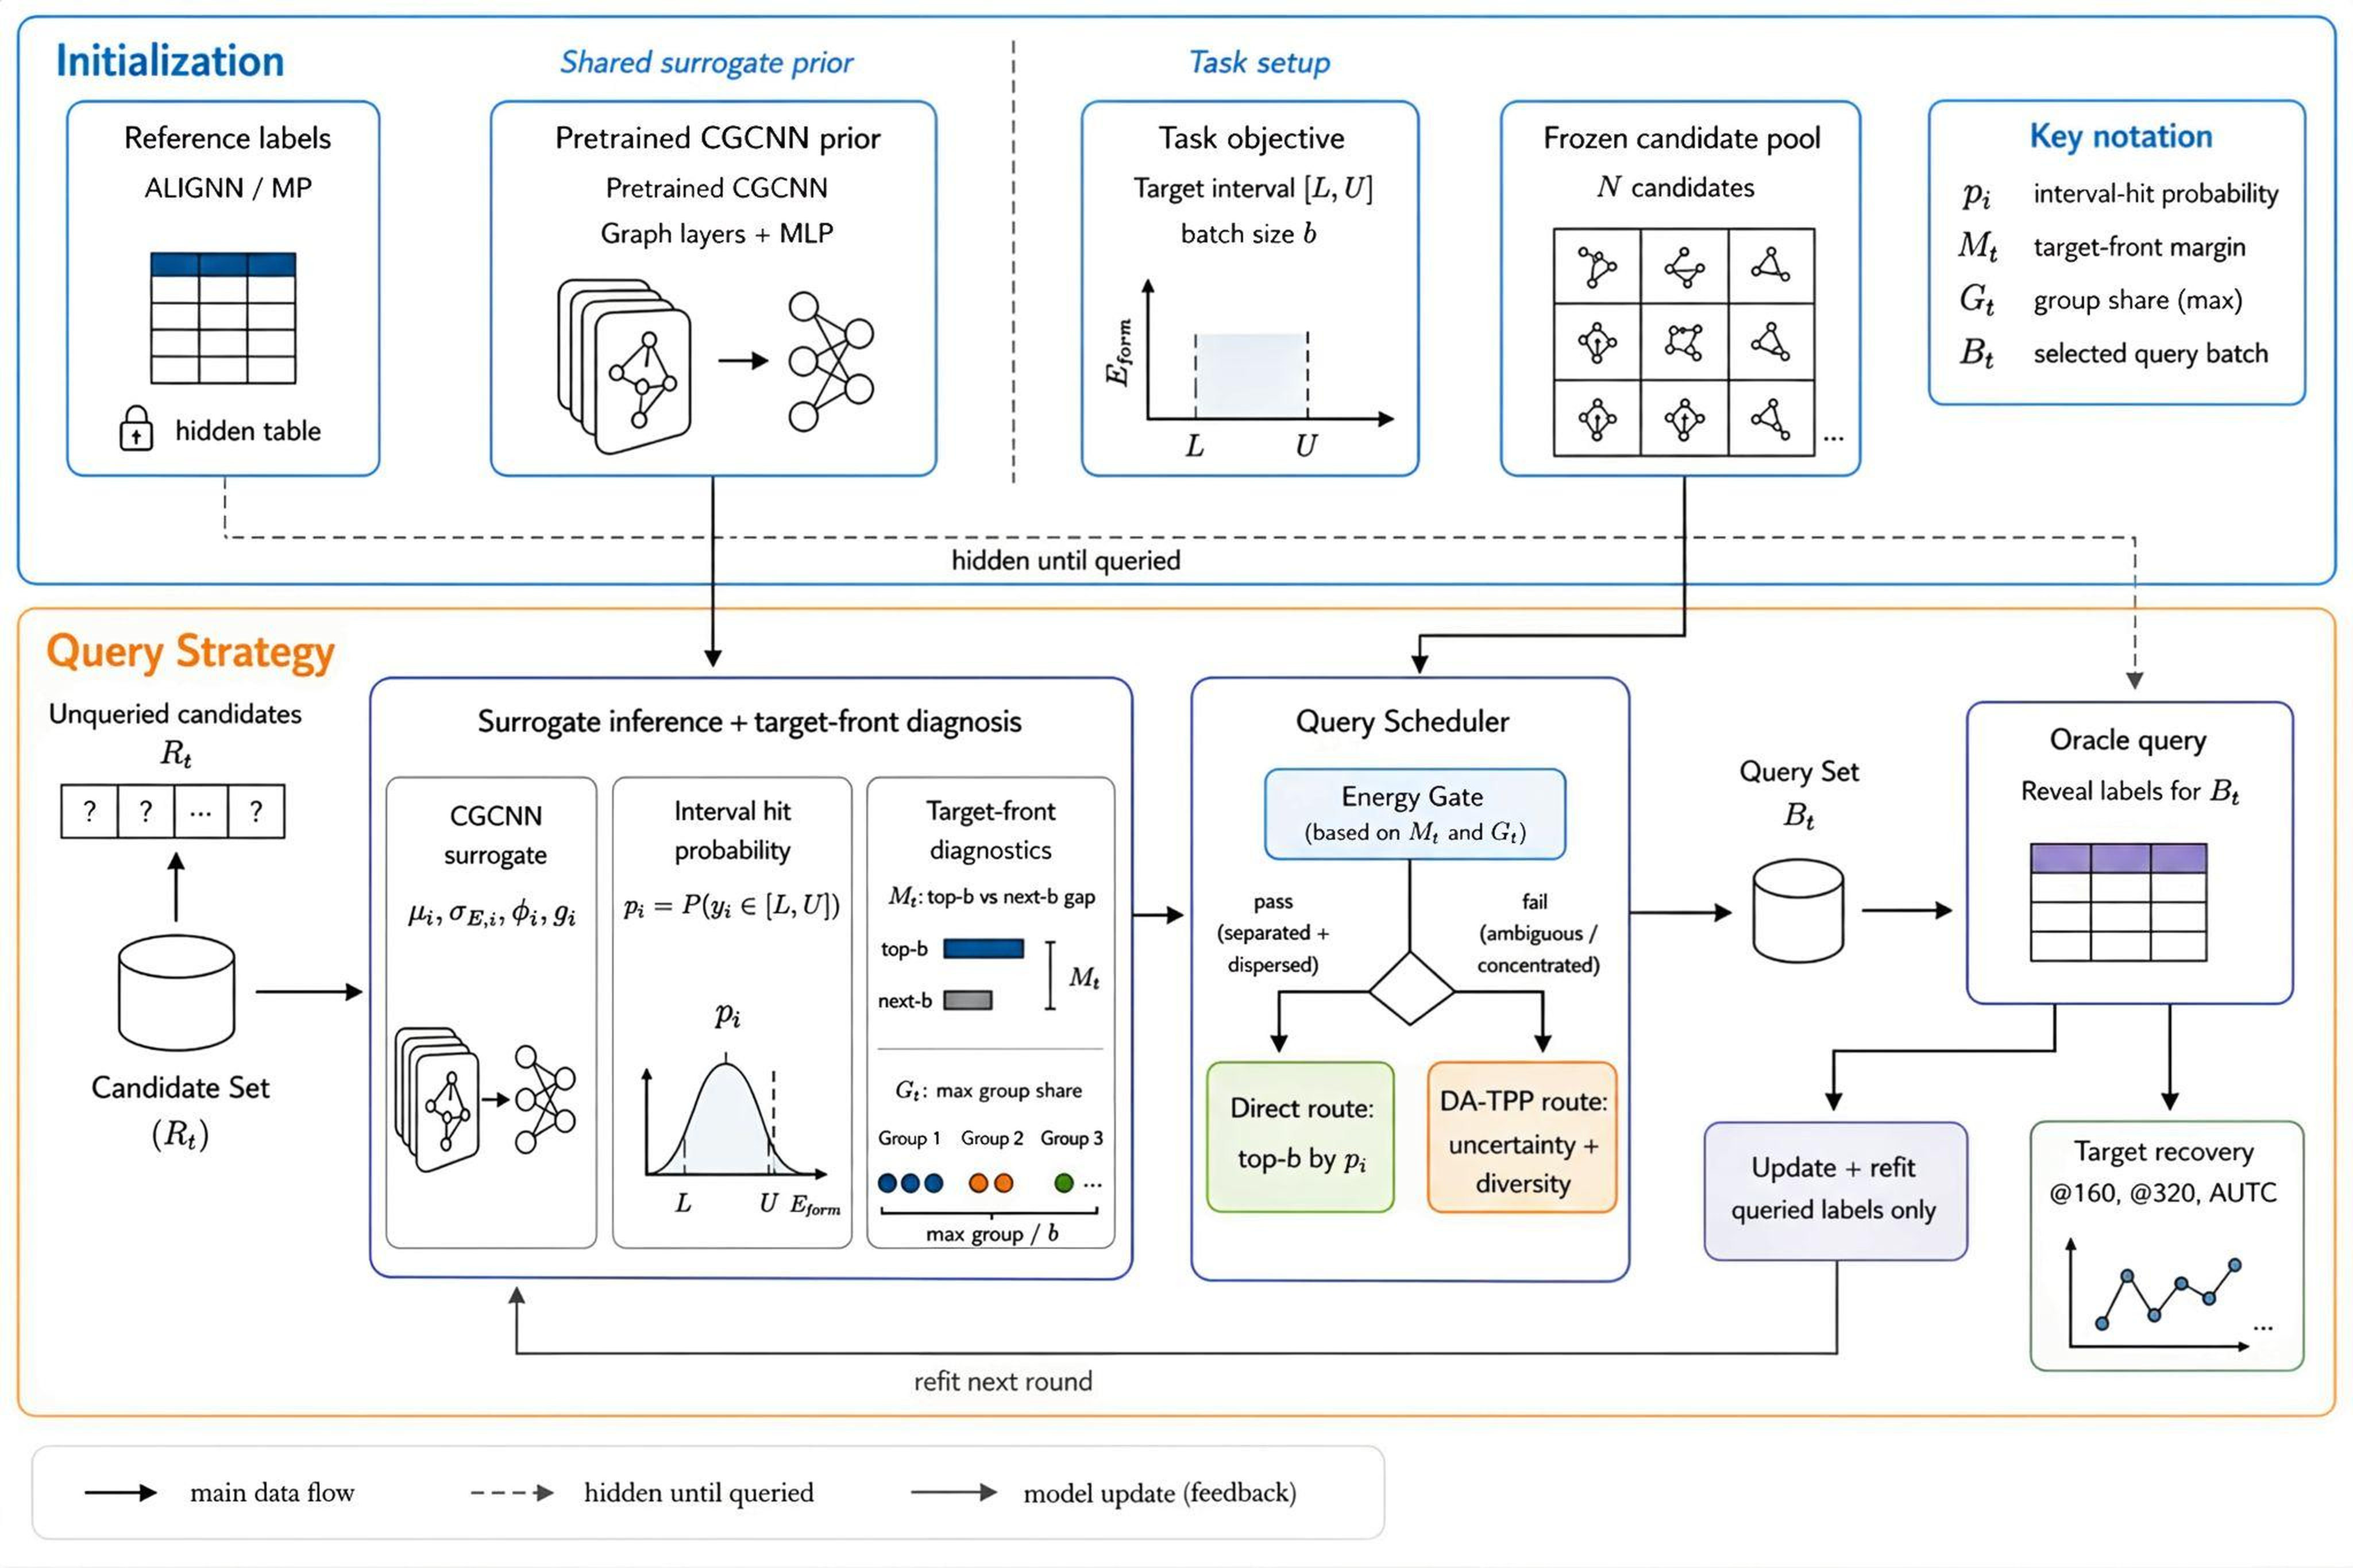
\includegraphics[width=0.90\textwidth]{Figure1_user_supplied_workflow_600dpi.png}
\caption{Workflow of Energy-Gated DA-TPP. Reference labels remain hidden until
queried. CGCNN predictions provide interval-hit probabilities and target-front
diagnostics; the gate retains the direct top-$b$ route or invokes
diversity-aware batch reconstruction before querying and refitting.}
\label{fig:acquisition-architecture}
\end{figure}

CGCNN predictions and newly revealed labels determine both stored histories.
MLIP outputs, evaluator scores, and DFT files are read only after a query
sequence has been fixed.

\subsection{Frozen candidate pool and surrogate target task}

This archive contains 640 MatterGen-derived Li--M--O spinel-like
candidates. Structures, the ALIGNN-derived label table, and query histories are
all frozen. Seventy-eight labels fall in $[-2.18,-2.02]$ eV atom$^{-1}$ and
define the surrogate target set. The interval belongs to this replay and is not
a threshold for phase stability or a materials application.

MatterGen records the origin of the generated pool, and the recoverable request
information is included in the Supplementary Material. No conversion has been
established among the generation request, the ALIGNN label convention, and the
formation energies calculated in the present DFT protocol.

Acquisition runs over the complete pool, which includes Cr-, Mn-, and
Mg-containing targets. For candidate $i$, MC dropout on the CGCNN gives mean
$\mu_i$ and standard deviation $\sigma_i$. The probability assigned to the
interval $[L,U]$ is
\begin{equation}
p_i =
\Phi\!\left(\frac{U-\mu_i}{\sigma_i+\epsilon}\right)
-\Phi\!\left(\frac{L-\mu_i}{\sigma_i+\epsilon}\right),
\label{eq:interval-hit}
\end{equation}
where $\Phi$ denotes the standard normal cumulative distribution function and
$\epsilon$ avoids division by zero. Predicted-Target Greedy takes the $b$
largest $p_i$ values in each round. It does not use either gate diagnostic or
any diversity term.

\subsection{Energy-gated batch acquisition}

Energy-Gated DA-TPP begins with that same top-$b$ list. It then inspects score
separation and chemical concentration at the current front. The margin statistic
compares the mean score of the leading batch with that of the next batch, using
the score variation across both batches as its scale:
\begin{equation}
M_t =
\frac{\operatorname{mean}_{i\in T_t^{(b)}}(p_i)
-\operatorname{mean}_{i\in T_t^{(2b)}\setminus T_t^{(b)}}(p_i)}
{\operatorname{sd}_{i\in T_t^{(2b)}}(p_i)+10^{-8}}.
\label{eq:margin}
\end{equation}
Group concentration is the largest fraction of the direct leading batch
assigned to a single chemical group:
\begin{equation}
G_t=\max_{g\in\mathcal{G}}
\frac{|\{i\in T_t^{(b)}:g_i=g\}|}{b}.
\label{eq:group-concentration}
\end{equation}
For this pool, the group key is the remaining metal label after Li and O are
removed from the composition.

Gate keeps the direct list when $M_t\ge M_0$ and $G_t\le G_0$. If either test
fails, candidates are placed into a new batch sequentially according to
\begin{equation}
s_i=p_i+\alpha\widetilde{\sigma}_{E,i}-\beta S_i-\gamma R_i,
\label{eq:correction}
\end{equation}
Here $\widetilde{\sigma}_{E,i}$ is normalized predictive spread. The term $S_i$
penalizes proximity to candidates already placed in the batch in the learned
representation, and $R_i$ penalizes reuse of the same chemical group.

Every recovered run configuration uses the same settings. Their values appear
in Supplementary Table~S2. The archive does not
contain a complete hyperparameter-development log, so these values are reported
as implementation settings rather than the outcome of an independent
optimization study.

\paragraph{Implementation sequence and complexity.}
Each round scores the unqueried pool, forms the direct top-$b$ batch, and
computes $M_t$ and $G_t$. Gate then accepts that batch or rebuilds it with
Eq.~\eqref{eq:correction}. The new labels are revealed only after the batch has
been selected, and the CGCNN is then refitted. Maintaining the leading lists
requires $O(N\log b)$ work per round. When correction is active, updating
representation distances costs $O(bNd)$ for embedding dimension $d$ and uses
$O(Nd)$ memory. These costs do not include the CGCNN refit common to both
policies. Full Gate and Group-only Gate have the same saved sequence, whereas
Margin-only follows Greedy. Thus the margin test did not independently alter
the route recorded in this archive.

\section{Experimental Protocol}

\subsection{Archived CGCNN protocol and run audit}

Across Gate and Greedy, the pool, reference labels, candidate order, initial
CGCNN checkpoint, batch size, query budget, and refitting schedule are held
constant. The policies differ only in how they assemble a batch. The archived CGCNN has
64-dimensional atom features, 128 hidden features, three graph-convolution
layers, and one hidden fully connected layer. After every acquisition round,
the model is refitted for 10 epochs using the labels accumulated by that policy.
Training uses a learning rate of 0.001 and batches of 256. Three MC-dropout
passes are made at dropout rate 0.30 \cite{ref-mcdropout}.

Each policy directory contains ten stored records associated with
implementation seeds 5--14. They are indexed as run IDs 1--10 in the paper, and
the mapping is supplied with the source. Hashes of the complete prefixes are
identical within a policy through 240 queries. By 320 queries, some non-target
positions differ, but the recovered target set is unchanged. Consequently, the
early-budget comparison consists of one distinct Gate path and one distinct
Greedy path. The stored IDs cannot support a repeated-run interval or a
significance test.

\subsection{Historical DFT-evaluability labels}

Twenty historical Cr-, Mn-, or Mg-containing candidates have traceable DFT
attempts. Ten satisfy the strict endpoint, which requires evidence of
electronic and ionic convergence, a separate static calculation, and a
reproducible formation energy. Among the ten records labelled zero, seven do
not preserve enough information to reconstruct the formation energy, two
contain a VASP or electronic failure, and one has an unconverged static step.
The negative class therefore denotes either observed workflow failure or
insufficient archived evidence under the stated protocol, rather than intrinsic
non-computability.
Candidate identity, acquisition rank, and evaluator output were excluded from
label assignment.

\subsection{First-principles feasibility protocol}

Four generated LiCr$_2$O$_4$ candidates were examined with first-principles
calculations: C079-1, C126-0, C196-1, and C234-3. These candidate-level
feasibility records are analysed separately from the Gate--Greedy acquisition
comparison.

All four calculations used VASP 6.5.1, PAW-PBE datasets, and the Dudarev
PBE+$U$ formulation \cite{ref-vasp,ref-paw,ref-paw-vasp,ref-pbe,ref-dudarev}.
The Cr value was $U_{\mathrm{eff}}=3.7$ eV, and the plane-wave cutoff was 649 eV.
Relaxations used \texttt{EDIFF}$=10^{-6}$ eV,
\texttt{EDIFFG}$=-0.05$ eV \AA$^{-1}$, \texttt{IBRION}$=2$,
\texttt{ISIF}$=3$, and \texttt{NSW}$=200$. Spin polarization was retained with
\texttt{ISMEAR}$=0$, \texttt{SIGMA}$=0.05$ eV, \texttt{LASPH}=TRUE, and
\texttt{LMAXMIX}$=4$. The relaxed cells were passed to separate static jobs
using \texttt{IBRION}$=-1$ and \texttt{NSW}$=0$. Candidate-specific meshes,
generated at approximately 0.15~\AA$^{-1}$ reciprocal spacing, are listed in the
Supplementary Material.

Formation energies were recalculated from compound and elemental reference
jobs run with the same protocol:
\begin{equation}
E_f=
\frac{E_{\mathrm{compound}}-\sum_j n_jE_j^{\mathrm{ref}}}
{\sum_j n_j}.
\label{eq:dft-formation-energy}
\end{equation}
The Supplementary Material gives the Li, Cr, and O$_2$ reference energies.
Independent scripts reproduced the formation energies to within
$10^{-15}$ eV atom$^{-1}$, verifying the arithmetic within the DFT convention.
Because no validated mapping to the ALIGNN labels is available, these formation
energies remain a separate evidence layer.

\subsection{Dual-MLIP computational layer and interpretation boundary}

CHGNet and MACE-MP were both run on all 640 structures. The 1,280 resulting
records include energies, forces, stresses, geometry changes, elapsed time, and
the disagreement between models. They are MLIP outputs rather than
PAW--PBE+$U$ observations. Ten historical records retain reconstructable DFT
energies. In each outer leave-one-out fold, nine of them determine a
composition-dependent offset and a nominal prediction interval, which are then
applied to the held-out record. Only those held-out predictions enter the MAE,
RMSE, and coverage calculations.

These records quantify low-fidelity prediction error and interval coverage for
the frozen pool. Because they were generated after the archived acquisition
runs, they are not used to estimate prospective DFT savings. Electronic,
magnetic, and thermodynamic properties are evaluated separately from this MLIP
comparison.

\subsection{DFT-evaluability model}

The evaluator uses 20 labelled records, so the comparison was restricted to
low-complexity classifiers. Every candidate had previously been
processed by the published CHGNet \cite{ref-chgnet} and MACE-MP
\cite{ref-macemp} models. Input features cover metal composition, atom count,
space-group number, original cluster size, minimum distance, and volume per
atom. Initial and final MLIP energies, maximum force, stress, volume change,
displacement, final space group, and cross-model disagreements are included as
well. Candidate IDs and archived acquisition ranks are not permitted features.

Four classifier families were compared: regularized logistic regression,
Laplace-approximated logistic regression, shallow random forest, and shallow
gradient boosting \cite{ref-randomforest,ref-gradientboosting,ref-sklearn}.
Preprocessing and model selection were repeated inside every outer training
fold of nested leave-one-out cross-validation. After this comparison, shallow
gradient boosting was fitted to all 20 development records to score candidates
without historical labels. The 20 labelled candidates retain their out-of-fold
probabilities, and the fixed threshold for a binary prediction is 0.50.

The model output
\begin{equation}
e_i=P_i(\text{strictly DFT-evaluable})
\label{eq:evaluable-prob}
\end{equation}
is an acquisition-blind model estimate of whether the strict archive rule will
be met. It is distinct from both an observed DFT outcome and a formation-energy
prediction.

\subsection{Formal DFT-evaluability endpoints}

For a policy prefix $\mathcal{S}_a(q)$, the expected number of targets meeting
the evaluator rule is
\begin{equation}
H_a(q)=\sum_{i\in\mathcal{S}_a(q)} z_i e_i .
\label{eq:evaluability-expected}
\end{equation}
A thresholded version counts only target candidates with $e_i\geq0.50$:
\begin{equation}
\widehat{H}_a(q)=
\sum_{i\in\mathcal{S}_a(q)}
z_i\,\mathbb{I}(e_i\ge 0.50).
\label{eq:evaluability-thresholded}
\end{equation}
Both quantities were evaluated at 80, 160, 240, and 320 queries. They describe
the model-estimated workflow evaluability of surrogate targets already chosen
by the original CGCNN policies. These scores are computed after selection and
never enter the acquisition rule.

Normalized area under the target-recovery curve summarizes the ordering up to a
chosen stopping budget $Q^\star$:
\begin{equation}
\operatorname{AUTC}_{Q^\star}=
\frac{b}{Q^\star T}\sum_{r=0}^{Q^\star/b-1}Y(rb),
\quad Q^\star\in\{80,160,240,320\},
\label{eq:autc}
\end{equation}
Here $b=16$, $T=78$, and $Y(q)$ is cumulative target recovery after $q$
queries. The left-continuous convention credits a target only after its batch
has returned. Values are reported at four stopping budgets so that an early
ordering difference is not hidden by the common 78-target ceiling. Once
recovered, a target contributes to every subsequent ordinate of the cumulative
curve; earlier discovery therefore increases AUTC even when two policies reach
the same final recovery.

\subsection{Legacy baselines and result types}

The archive provides six-policy context through one complete query order for
Explore, the Modulus/Gradient-Norm hybrid, MC Dropout, and Random Sampling,
together with an earlier Gate--Greedy pair. All six orders use the same
surrogate target table. Because each policy contributes one order rather than
matched repeats, the comparison is reported descriptively.

Greedy sorts the interval-hit probability. Explore adds coverage in learned
representation space within a prediction-preferred front. MC Dropout orders
candidates by predictive uncertainty, and the Modulus/Gradient-Norm method
combines gradient magnitude with target-directed selection. Random Sampling
follows one archived random order. Figure~\ref{fig:six-policy-benchmark} plots
their recovery histories, and Supplementary Table~S8 gives the checkpoints and
DFT-evaluability overlay.

Counts taken directly from CGCNN histories or DFT files are referred to as
observed, whereas values produced by the DFT-evaluability model are marked as
ML-estimated. Application-specific properties and experimental synthesizability
are outside the present endpoints.

\subsection{Materials Project Mn-oxide control}

The database-derived control contains 640 Mn-bearing oxides with Materials
Project formation energies as reference labels. Its fixed target interval,
$[-2.59,-2.47]$ eV atom$^{-1}$, contains 111 candidates. Gate and Greedy were
run in ten corrected seed pairs (seeds 5--14) with batch size 16, a 320-query
budget, candidate-ID reindexing, and prediction-loader shuffling disabled. The
two policies shared the same seed-specific training and inference schedule.

The control uses a label-blind sorted element-system key. This map contains 614
groups among the 640 candidates, including 588 singleton groups, and no group
contains more than two candidates. The control therefore tests the behaviour of
the gate when the direct batch has little group-level redundancy. Candidate
maps, per-seed metrics, and the pairing audit are reported in Supplementary
Table~S11 and the accompanying source files.

\subsection{Development and held-out evaluation protocol}

Gate sensitivity was evaluated without retroactively changing the archived main
result.
On development seeds 0--4, a $3\times3$ threshold grid crossed
$M_0\in\{0.75,1.00,1.25\}$ with
$G_0\in\{0.40,0.50,0.60\}$. A separate one-factor sweep retained
$M_0=1.00$ and $G_0=0.50$ while varying
$\alpha\in\{0.05,0.20\}$, $\beta\in\{0.10,0.40\}$, or
$\gamma\in\{0.05,0.20\}$ around the archived
$(\alpha,\beta,\gamma)=(0.10,0.20,0.10)$. All runs used 30 MC-dropout passes,
batch size 16, the fixed 640-candidate pool, and the same refitting schedule.
The grid was analysed as a parameter-response surface. Because $\gamma=0.05$ gave the
highest development-cohort AUTC through 160 queries among the tested group-reuse
weights, this single value was carried forward while $M_0$, $G_0$, $\alpha$, and
$\beta$ remained unchanged. The resulting protocol was locked before any result
from held-out seeds 15--24 was inspected. These ten seeds used different initial
labelled sets, and the primary held-out endpoint was normalized AUTC through 160
queries. Configuration, run, metric, and trajectory hashes were recorded for all
20 Gate--Greedy runs.

The same development protocol was also run for Predicted-Target Greedy, MC
Dropout, and Random Sampling. These low-cost controls test whether Gate's early
gain persists when stochasticity, dropout count, pool, budget, and refitting are
aligned. They supplement rather than overwrite the
six archived histories. Per-configuration and per-method source results are
reported in Supplementary Tables~S12--S13. The held-out configuration,
per-seed values, and pairing audit are reported in Supplementary Table~S14 and
the accompanying source files.

\section{Experiments and Results}

\subsection{Legacy six-policy comparison}

The descriptive archive first places the proposed policy beside the five
previously implemented selectors under a common surrogate target table. The
complete recovery curves are shown before the protocol-matched Gate--Greedy
analysis so that the relative early-budget behaviour of all six policies remains
visible.

\begin{figure}[!htbp]
\centering
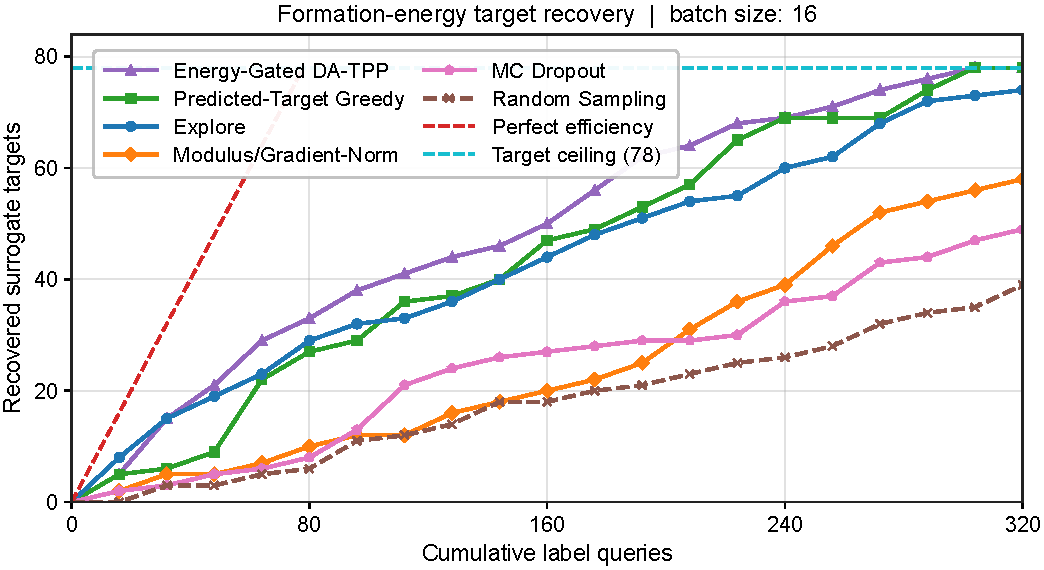
\includegraphics[width=0.86\textwidth]{Figure2_v50_six_policy_mentor.pdf}
\caption{Target recovery in the six archived policy histories. Markers denote
the 16-query batch checkpoints. The red dashed segment is perfect query
efficiency up to the 78-target ceiling, shown in cyan.}
\label{fig:six-policy-benchmark}
\end{figure}

Gate recovered the most targets at the early checkpoints of this archive. After
80 queries, its count was 33, compared with 29 for Explore and 27 for Greedy;
the corresponding counts for Modulus/Gradient-Norm, MC Dropout, and Random
Sampling were 10, 8, and 6. At 160 queries, the six counts in the same order
were 50, 44, 47, 20, 27, and 18. Gate and Greedy each reached 69 targets at 240
queries and the full set of 78 at 320. Each curve is one archived order, so this
panel is a broad method comparison rather than a repeated-run statistical test.
The exact checkpoints and the evaluator overlay are provided
in Supplementary Table~S8.

\subsection{Nested leave-one-out assessment of DFT evaluability}

The post-selection evaluator was tested before it was applied to acquisition
prefixes. Table~\ref{tab:evaluator-validation} compares four deliberately small
classifiers under nested leave-one-out assessment of the 20 historical DFT
attempts.

\begin{table}[!htbp]
\centering
\caption{Nested leave-one-out assessment of the DFT-evaluability classifiers.}
\label{tab:evaluator-validation}
\scriptsize
\begin{tabular}{lrrrr}
\toprule
Model & ROC--AUC & Balanced accuracy & Brier score & Log loss \\
\midrule
Shallow gradient boosting & 0.820 & 0.700 & 0.183 & 0.545 \\
Shallow random forest & 0.660 & 0.750 & 0.234 & 0.664 \\
Regularized logistic regression & 0.540 & 0.600 & 0.258 & 0.713 \\
Laplace logistic model & 0.460 & 0.600 & 0.282 & 0.766 \\
\bottomrule
\end{tabular}
\tabnote{The development archive contains 20 DFT attempts, including 10
strictly evaluable records. Preprocessing and model selection are performed
inside each outer training fold.}
\end{table}


Shallow gradient boosting gave the highest ROC--AUC (0.820), as well as the
lowest Brier score and log loss. Within this development archive, the ROC value
means that an evaluable record received the higher score in 82\% of the
positive--negative pairs represented by the calculation. Random forest produced
the best balanced accuracy at the fixed 0.50 threshold, but the stronger
probability ranking and probability losses of gradient boosting made it the
model used for $e_i$. Candidate-level labels and outer-fold probabilities are
available in Supplementary Section~S4.

\subsection{Gate--Greedy target recovery}

The primary comparison uses the corrected, protocol-matched Gate and Greedy
histories. Figure~\ref{fig:gate-greedy-evidence} reports cumulative recovery,
the separate DFT-evaluability audit, and normalized AUTC at four stopping
horizons.

\begin{figure}[!htbp]
\centering
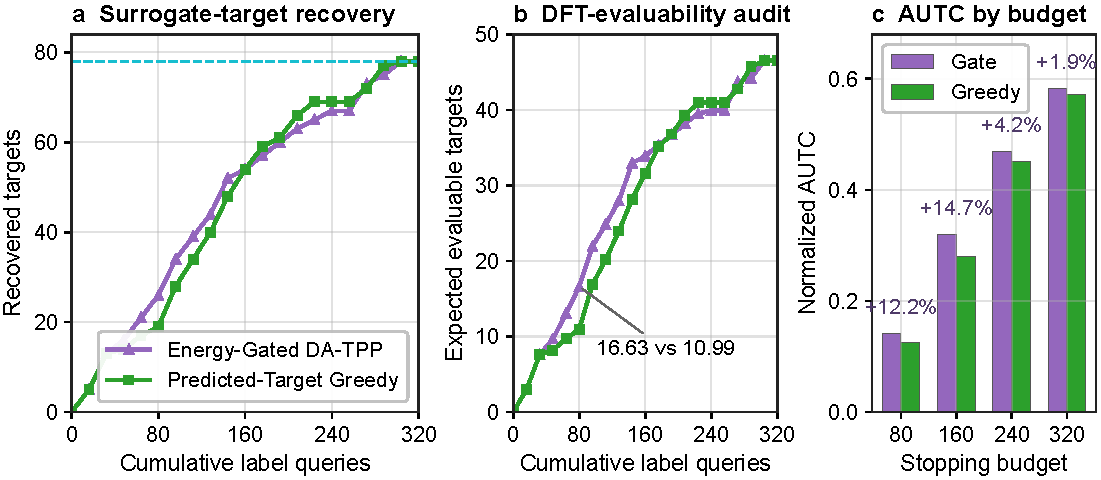
\includegraphics[width=0.90\textwidth]{Figure3_v50_gate_greedy_evidence.pdf}
\caption{Gate and Greedy under the matched replay protocol. (a) Cumulative
recovery of 78 reference targets. (b) Expected DFT-evaluable target count from
the post-selection metric. (c) Normalized AUTC at four stopping budgets,
with labels showing Gate relative to Greedy. Each method contributes one
distinct early query path.}
\label{fig:gate-greedy-evidence}
\end{figure}

Gate recovered 26 targets in the first 80 queries, compared with 19 for Greedy,
an increase of seven targets or 36.8\%. The two paths were tied at 54 after 160
queries; Greedy then held a 69--67 lead at 240, and both reached all 78 targets
by 320. Normalized AUTC retains the early placement: Gate obtained 0.1410,
0.3205, 0.4692, and 0.5827 through 80, 160, 240, and 320 queries, whereas Greedy
obtained 0.1256, 0.2795, 0.4504, and 0.5718. The largest relative advantage was
14.7\% through 160 queries and narrowed as the common endpoint approached.

The stored IDs within each policy share the same prefix through 240 queries;
they therefore describe one distinct early trajectory per method. The prefix
hash audit is reported in Supplementary Table~S6, and the stopping-horizon AUTC
calculation is reported in Supplementary Table~S7.

\subsection{DFT evaluability of selected targets}

Table~\ref{tab:evaluability-yield} applies the evaluator only after each query
prefix has been fixed. It separates observed ALIGNN target hits from the summed
and thresholded DFT-evaluability estimates.

\begin{table}[!htbp]
\centering
\caption{Surrogate target recovery and the formal DFT-evaluability endpoint at the
fixed query checkpoints.}
\label{tab:evaluability-yield}
\scriptsize
\begin{tabular}{llrrrr}
\toprule
Queries & Method & Target hits & Expected evaluable & $e_i\geq0.50$ & Mean $e_i$ \\
\midrule
80  & Gate   & 26 & 16.63 & 20 & 0.64 \\
    & Greedy & 19 & 10.99 & 12 & 0.58 \\
160 & Gate   & 54 & 33.87 & 41 & 0.63 \\
    & Greedy & 54 & 31.60 & 35 & 0.59 \\
240 & Gate   & 67 & 39.93 & 46 & 0.60 \\
    & Greedy & 69 & 40.96 & 47 & 0.59 \\
320 & Gate   & 78 & 46.51 & 53 & 0.60 \\
    & Greedy & 78 & 46.51 & 53 & 0.60 \\
\bottomrule
\end{tabular}
\tabnote{Expected evaluable is $\sum z_i e_i$ over the targets already selected
by the CGCNN policy. The acquisition-blind $e_i$ values are ML estimates and are
not supplied to Gate or Greedy.}
\end{table}


At 80 queries, Gate's 26 targets summed to an expected evaluable count of 16.63,
whereas Greedy's 19 targets summed to 10.99. Thresholding at 0.50 gave 20 and 12
candidates, respectively. The early prefix favoured by target recovery was thus
also assigned the larger downstream evaluability total by a model that did not
participate in acquisition. The expected counts were 33.87 and 31.60 at 160
queries; Greedy led 40.96 to 39.93 at 240; and the two values converged to 46.51
when both methods had found all 78 targets. These are post-selection estimates,
not outcomes from newly submitted DFT jobs. Full candidate-level values are
reported in Supplementary Section~S5.

\subsection{Full-pool MLIP execution and DFT comparison}

CHGNet and MACE-MP each completed all 640 candidates, yielding 1,280
low-fidelity records. Their combined recorded wall time was 781.5 s, with median
times of 0.58 s per candidate for CHGNet and 0.41 s for MACE-MP. The complete
runtime distributions and source values are given in Supplementary Figure~S1.

For the ten records with reconstructable DFT energies, leave-one-out offset
correction produced an MAE of 0.0145 eV atom$^{-1}$ and an RMSE of
0.0159 eV atom$^{-1}$. Figure~\ref{fig:mlip-calibration} shows each outer-fold
prediction rather than an in-sample fit. Seven DFT values lay inside the nominal
95\% intervals; interval calibration is therefore interpreted at the scale of
this ten-record comparison.

\begin{figure}[!htbp]
\centering
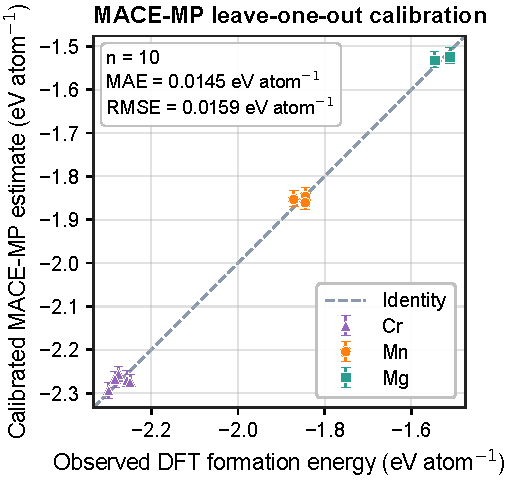
\includegraphics[width=0.55\textwidth]{Figure4_v50_mace_dft_calibration.pdf}
\caption{Leave-one-out offset correction of MACE-MP predictions for ten
reconstructable DFT formation energies. Points show outer-fold predictions and
vertical bars show nominal 95\% intervals. Colours distinguish Cr-, Mn-, and
Mg-containing records.}
\label{fig:mlip-calibration}
\end{figure}

\subsection{Route attribution within the stored ablations}

Sequence hashes attribute the archived reordering to the group-triggered
branch. Full Energy-Gated DA-TPP and Group-only Gate chose the same candidates
in the same order, whereas Margin-only reproduced Greedy. Group-triggered
correction, rather than the margin condition, therefore caused the recorded
sequence change.

\subsection{Crystallographic and first-principles assessment}

The four completed LiCr$_2$O$_4$ workflows show that generated candidates from
the pool can retain compact structures after cell-and-ion relaxation and
complete independent static calculations. Figure~\ref{fig:dft-feasibility}
compares the relaxed cells, while Table~\ref{tab:dft-candidates} connects their
geometry to the independently reconstructed formation energies and electronic
diagnostics.

\begin{figure}[H]
\centering
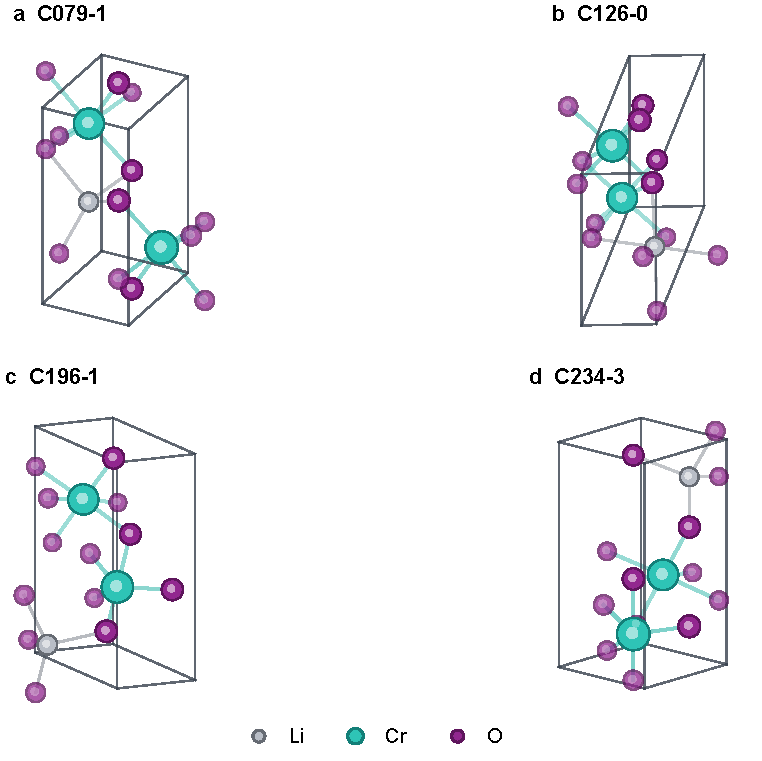
\includegraphics[width=0.70\textwidth]{Figure5_v50_relaxed_structures.pdf}
\caption{Relaxed LiCr$_2$O$_4$ cells used for independent static calculations:
(a) C079-1, (b) C126-0, (c) C196-1, and (d) C234-3. The cells were reconstructed
from final \texttt{vasprun.xml} files. Li--O and Cr--O segments indicate local
coordination only; no bond order is assigned.}
\label{fig:dft-feasibility}
\end{figure}

The corresponding numerical descriptors are summarized below. Each row refers
to a completed relaxation followed by a separate static calculation under the
same PAW--PBE+$U$ protocol.

\begin{table}[H]
\centering
\caption{Geometry, formation energy, magnetic moment, and near-zero gap for the
four completed LiCr$_2$O$_4$ workflows.}
\label{tab:dft-candidates}
\tablesize{\scriptsize}
\resizebox{\textwidth}{!}{\begin{tabular}{@{}lrrrrrr@{}}
\toprule
Candidate & $E_f$ (eV atom$^{-1}$) & $F_{\max}$ (eV \AA$^{-1}$) &
$\Delta V$ (\%) & Shortest distance (\AA) &
Moment ($\mu_{\mathrm{B}}$ cell$^{-1}$) & Gap (eV) \\
\midrule
C079-1 & $-2.164905884$ & 0.045128 & $+2.918$ & 1.917646 & 4.937 & 0.0035 \\
C126-0 & $-2.167618531$ & 0.034407 & $-1.358$ & 1.938847 & 4.922 & 0.0010 \\
C196-1 & $-2.033635033$ & 0.033610 & $+0.962$ & 1.724317 & 4.864 & 0.0004 \\
C234-3 & $-2.033665270$ & 0.044104 & $+0.586$ & 1.724466 & 4.864 & 0.0015 \\
\bottomrule
\end{tabular}
}
\tabnote{Gap values come from one PBE+$U$ protocol. Magnetic moments refer to
the tested initialization for each candidate.}
\end{table}

All four relaxations met the 0.05 eV~\AA$^{-1}$ force criterion, with
$F_{\max}=0.033610$--0.045128 eV~\AA$^{-1}$. Their volume changes remained
between $-1.358\%$ and $+2.918\%$, final cell volumes spanned only
73.810--75.547~\AA$^3$, and the shortest interatomic distances were
1.7243--1.9388~\AA. The four structures therefore retained compact,
non-collapsed seven-site cells despite their visibly different lattice shapes.

Automated symmetry analysis further distinguishes the relaxed candidates. At a
0.10~\AA\ symmetry tolerance, C079-1, C126-0, C196-1, and C234-3 were assigned
to Pmm2, C2/m, R3m, and P3m1, respectively. A composition-preserving
StructureMatcher comparison found no matching pair under the recorded
tolerances. Thus the four panels represent distinct relaxed structural variants
rather than duplicate drawings of one cell. Lattice parameters, symmetry
tolerance checks, pairwise matching settings, and CIF hashes are reported in
Supplementary Table~S10.

The energetic results also form two closely clustered groups. C079-1 and C126-0 lie
near $-2.166$ eV atom$^{-1}$, while C196-1 and C234-3 lie near
$-2.034$ eV atom$^{-1}$. The latter pair differs by only 0.030 meV
atom$^{-1}$ and is not ranked against each other. Final moments span
4.864--4.937 $\mu_{\mathrm B}$ per cell, and all four PBE+$U$ gaps are below
0.004 eV. Complete numerical settings, reference energies, restart provenance,
and final CIFs are listed in Supplementary Tables~S9--S10.

\section{Discussion and Limitations}

\subsection{Database-derived Mn-oxide control and Greedy fallback}

The Materials Project Mn-oxide control tests the complementary regime to the
generated Li--M--O pool. Its element-system representation is highly sparse:
614 groups describe 640 candidates, 588 groups are singletons, and the largest
group contains only two candidates. This geometry leaves almost no batch-level
repetition for the correction route to remove, favouring the direct ranking.
Table~\ref{tab:mnoxide-control} summarizes the paired control outcome;
checkpoint-level values for all ten seeds are reported in Supplementary
Table~S11.

\begin{table}[!htbp]
\caption{Mn-oxide fallback control across corrected seeds 5--14.}
\label{tab:mnoxide-control}
\centering
\small
\begin{tabular}{@{}ll@{}}
\toprule
Control diagnostic & Observed result \\
\midrule
Paired Gate--Greedy AUTC difference & 0 for all 10 seed pairs \\
Batch candidate sets & Identical for all 10 seed pairs \\
Gate routing & 199 direct; 1 correction batch \\
Effective candidate replacements & 0 \\
Final target recovery & Identical for Gate and Greedy \\
\bottomrule
\end{tabular}
\end{table}

The only correction event, in seed 5, changed within-batch order but not batch
membership. The zero paired AUTC differences and absence of effective
replacements identify a direct-ranking fallback under a group representation
with insufficient redundancy.

\subsection{Gate-parameter sensitivity}

The development-cohort sweep asks whether the routing interpretation depends on
a narrow parameter choice. Figure~\ref{fig:parameter-sensitivity} separates the
two diagnostic thresholds from the three diversity weights and reports both
early recovery and route activity across seeds 0--4.

\begin{figure}[!htbp]
\centering
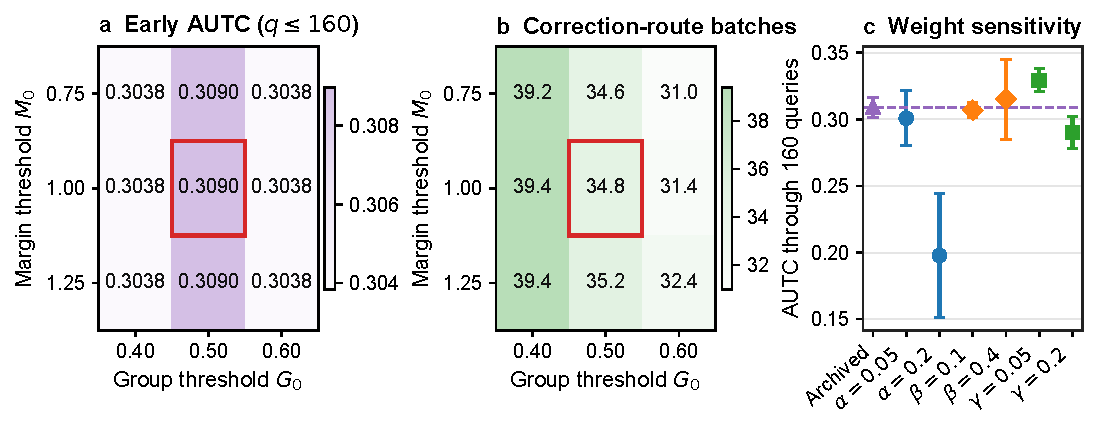
\includegraphics[width=0.95\textwidth]{Figure7_v63_parameter_sensitivity_light.pdf}
\caption{Development-cohort gate sensitivity with 30 MC-dropout passes.
(a) Mean normalized AUTC through 160 queries across the $M_0$--$G_0$ grid.
(b) Mean number of correction-route batches across the same grid. The red box
marks the archived thresholds. (c) One-factor sensitivity of AUTC through 160
queries to $\alpha$, $\beta$, and $\gamma$; points show means and bars show
sample SD across seeds 0--4.}
\label{fig:parameter-sensitivity}
\end{figure}

The archived setting and all configuration-level results are reported in
Supplementary Table~S12.

Across the threshold grid, mean AUTC through 160 queries occupied a narrow
0.3038--0.3090 band, and mean recovery at 80 queries ranged from 26.2 to 27.0
targets. The archived $G_0=0.50$ setting lay at the upper edge of that early
surface. Varying $M_0$ from 0.75 to 1.25 did not change early AUTC or checkpoint
recovery at fixed $G_0$, although it modestly changed some late route counts and
complete sequence hashes. Early AUTC is therefore insensitive to $M_0$ across
the tested range, whereas group concentration is the active diagnostic in the
recorded Li--M--O task.

The correction weights exerted a clearer influence. Aggressive uncertainty
weighting reduced early recovery, whereas the tested $\beta$ values remained
near the archived result. The best development mean, 0.3292, occurred at
$\gamma=0.05$; this value was fixed for the independent held-out comparison.
The complete sensitivity grid is reported in Supplementary Table~S12. The
same-protocol controls in Supplementary Table~S13 use the archived
$\gamma=0.10$ configuration; the development-selected $\gamma=0.05$ protocol
is evaluated separately in Supplementary Table~S14.

The held-out comparison addresses the repeated-prefix limitation of the
archive. Figure~\ref{fig:gamma005-holdout} shows all ten paired AUTC$_{160}$
observations and the checkpoint recovery means; numerical values and the pairing
audit are provided in Supplementary Table~S14.

\begin{figure}[!htbp]
\centering
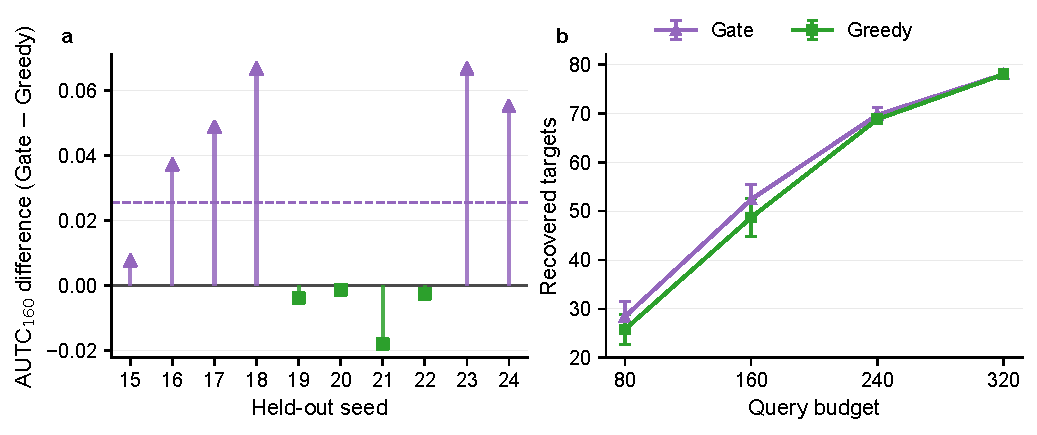
\includegraphics[width=0.95\textwidth]{Figure7_v69_gamma005_holdout_clean.pdf}
\caption{Frozen held-out comparison on independently initialized seeds 15--24.
(a) Per-seed difference in normalized AUTC through 160 queries; values above
zero favour Gate, values below zero favour Greedy, and the dashed line marks
the cohort mean of $+0.0256$. (b) Mean target recovery at the four prespecified
stopping budgets; error bars show sample SD across ten seeds. Purple triangles
denote Gate and green squares denote Greedy. All runs used the
development-selected $\gamma=0.05$, 30 MC-dropout passes, and otherwise
unchanged parameters.}
\label{fig:gamma005-holdout}
\end{figure}

Gate increased mean AUTC$_{160}$ by 0.0256, or 8.6\% relative to Greedy, and
increased mean recovery by 2.6 targets at 80 queries and 3.7 targets at 160
queries. The paired bootstrap interval for the AUTC$_{160}$ difference was
[0.0067, 0.0449], while the exact two-sided Wilcoxon test gave $p=0.105$ and
$d_z=0.789$. Six seed pairs favoured Gate and four favoured Greedy. The positive
differences were larger in magnitude on average than the negative differences,
producing a positive cohort mean despite non-uniform pairwise outcomes. The
bootstrap interval estimates the mean paired difference, whereas the exact
Wilcoxon test assesses paired ranks; with ten pairs, the two summaries need not
give identical inferential conclusions. Ten unique sequence hashes per method
confirm that these are distinct query trajectories rather than duplicate
prefixes.

\subsection{Mechanism and practical budget analysis}

Across the archived and held-out comparisons, the gain is concentrated before
the common final ceiling. This is the regime in which ordering matters: a
campaign may stop early or launch expensive calculations from an interim
shortlist. Gate retains the Greedy front unless the group diagnostic identifies
redundancy, so the added coverage does not replace the exploitation baseline.

The sequence hashes and Mn-oxide control attribute the observed route change to
group-triggered correction. Correction changes the generated-pool sequence,
whereas the sparse control map offers no effective replacement and returns the
Greedy path. This conditional behaviour explains how Gate can improve early
target yield without sacrificing the final recovery ceiling.

\subsection{Evidence scope and limitations}

Together, the held-out cohort and Mn-oxide control support two conclusions:
Gate improves mean early target ordering when removable group redundancy is
present, and it preserves the Greedy path when no effective replacement exists.
The archived early comparison provides supporting rather than replicated
evidence because its stored run IDs share query prefixes.

The post-selection evaluator extends the analysis toward workflow feasibility
but is trained on 20 historical attempts and does not enter acquisition. ALIGNN,
MLIP, and PAW--PBE+$U$ values remain distinct energy conventions. The four
LiCr$_2$O$_4$ calculations verify converged, structurally distinct candidates
under the stated protocol; phase stability and broader magnetic sampling are
outside the present study. Provenance and numerical details are reported in
Supplementary Tables~S9--S10.

\section{Conclusions and Future Work}

Energy-Gated DA-TPP conditionally adds diversity control to a strong Greedy
selector. In the archived 640-candidate replay, it recovered 26 targets within
80 queries versus 19 for Greedy. After development-only selection of
$\gamma=0.05$, the held-out cohort increased mean AUTC$_{160}$ from
0.2967 to 0.3223 and recovered more targets at both early checkpoints. Together,
the archived replay and held-out cohort show an aggregate early-budget
advantage while preserving the common final recovery ceiling.

The ablations attribute the observed reordering to group-triggered correction,
and the Mn-oxide control shows that Gate falls back to Greedy when no effective
replacement exists. An acquisition-blind post-selection audit assigned the
early Gate prefix greater predicted DFT evaluability, and four generated
LiCr$_2$O$_4$ candidates completed
the common PAW--PBE+$U$ relaxation--static workflow as distinct relaxed
structures. Future work will extend the comparison to prospective DFT outcomes,
competing-phase calculations, and broader magnetic-state sampling.


\acknowledgement{We also acknowledge Hubei University of Technology and the National ``111 Research Center'' for Microelectronics and Integrated Circuits for providing research facilities, and the University of Nottingham for providing relevant research software.}
\useofartificialintelligence{During the preparation of this work, the authors used OpenAI Codex to support language editing, LaTeX and reproducibility-package organization, figure-format checks, and pre-submission consistency checks. The authors reviewed and edited all affected material, verified the supporting data and references, and take full responsibility for the content of the article.}
\funding{This work was supported in part by the China Scholarship Council; the Innovation and Entrepreneurship Program for College Students of the Ministry of Education of China (Grant No. 20250100164); the Key Research Project of the Xinjiang Autonomous Region--Joint Task Special Project between Provincial Department and Local Government, China (Grant No. 20261152731); and the Innovation and Entrepreneurship Program for College Students of the Education Department of Hubei Province, China (Grant No. 20240200145).}
\authorcontributions{Yueyang Zhang and Jinxuan Liu contributed equally to conceptualization, methodology, software, validation, formal analysis, investigation, data curation, visualization, writing--original draft, and writing--review and editing. Tianyu Li: Validation, investigation, writing--review and editing. Xiangxiru Xiong: Validation, formal analysis, writing--review and editing. Yingjie Zhang: Validation, investigation, resources, writing--review and editing. Baohua Tan: Supervision, project administration, resources, funding acquisition, writing--review and editing. All authors reviewed the results and approved the final version of the manuscript.}
\availabilityofdataandmaterials{The submission package contains the frozen histories, figure source data, DFT-evaluability protocol and scores, MLIP calibration outputs, DFT audit table, final candidate structures, and figure-rebuild scripts. These materials are also available from the corresponding author upon reasonable request.}
\supplementary{The separate Supplementary Material contains additional protocol details, Figure~S1, Tables~S1--S14, candidate-level audits, and the reproducibility inventory in Supplementary Section~S17. The accompanying data-and-code package contains the cited source-data tables, figure-generation scripts, final candidate CIF files, environment specifications, and SHA-256 manifests.}
\ethicsapproval{Not applicable.}
\conflictsofinterest{The authors declare no conflicts of interest.}

\reftitle{References}
\begin{thebibliography}{99}
\bibitem{ref-cdvae} Xie T, Fu X, Ganea OE, Barzilay R, Jaakkola T. Crystal diffusion variational autoencoder for periodic material generation. Paper presented at: 10th International Conference on Learning Representations; 2022 Apr 25--29; Virtual.
\bibitem{ref-diffcsp} Jiao R, Huang W, Lin P, Han J, Chen P, Lu Y, et al. Crystal structure prediction by joint equivariant diffusion. Adv Neural Inf Process Syst. 2023;36:17464--97.
\bibitem{ref-mattergen} Zeni C, Pinsler R, Zuegner D, Fowler A, Horton M, Fu X, et al. A generative model for inorganic materials design. Nature. 2025;639:624--32. doi: 10.1038/s41586-025-08628-5.
\bibitem{ref-chemeleon} Park H, Onwuli A, Walsh A. Exploration of crystal chemical space using text-guided generative artificial intelligence. Nat Commun. 2025;16(1):4379. doi: 10.1038/s41467-025-59636-y.
\bibitem{ref-materials-project} Jain A, Ong SP, Hautier G, Chen W, Richards WD, Dacek S, et al. Commentary: The Materials Project: a materials genome approach to accelerating materials innovation. APL Mater. 2013;1(1):011002. doi: 10.1063/1.4812323.
\bibitem{ref-oqmd} Kirklin S, Saal JE, Meredig B, Thompson A, Doak JW, Aykol M, et al. The Open Quantum Materials Database (OQMD): assessing the accuracy of DFT formation energies. npj Comput Mater. 2015;1:15010. doi: 10.1038/npjcompumats.2015.10.
\bibitem{ref-aflow} Curtarolo S, Setyawan W, Hart GLW, Jahnatek M, Chepulskii RV, Taylor RH, et al. AFLOW: an automatic framework for high-throughput materials discovery. Comput Mater Sci. 2012;58:218--26. doi: 10.1016/j.commatsci.2012.02.005.
\bibitem{ref-jarvis} Choudhary K, Garrity KF, Reid ACE, DeCost B, Biacchi AJ, Hight Walker AR, et al. The joint automated repository for various integrated simulations (JARVIS) for data-driven materials design. npj Comput Mater. 2020;6:173. doi: 10.1038/s41524-020-00440-1.
\bibitem{ref-badge} Ash JT, Zhang C, Krishnamurthy A, Langford J, Agarwal A. Deep batch active learning by diverse, uncertain gradient lower bounds. Paper presented at: 8th International Conference on Learning Representations; 2020 Apr 26--30; Virtual.
\bibitem{ref-coreset} Sener O, Savarese S. Active learning for convolutional neural networks: a core-set approach. Paper presented at: 6th International Conference on Learning Representations; 2018 Apr 30--May 3; Vancouver, Canada.
\bibitem{ref-kmeanspp} Arthur D, Vassilvitskii S. k-means++: the advantages of careful seeding. In: Proceedings of the 18th Annual ACM-SIAM Symposium on Discrete Algorithms; 2007 Jan 7--9; New Orleans, LA, USA. p. 1027--35.
\bibitem{ref-localpenalization} Gonzalez J, Dai Z, Hennig P, Lawrence N. Batch Bayesian optimization via local penalization. In: Proceedings of the 19th International Conference on Artificial Intelligence and Statistics; 2016 May 9--11; Cadiz, Spain. Proc Mach Learn Res. 2016;51:648--57.
\bibitem{ref-cgcnn} Xie T, Grossman JC. Crystal graph convolutional neural networks for an accurate and interpretable prediction of material properties. Phys Rev Lett. 2018;120(14):145301. doi: 10.1103/PhysRevLett.120.145301.
\bibitem{ref-alignn} Choudhary K, DeCost B. Atomistic line graph neural network for improved materials property predictions. npj Comput Mater. 2021;7:185. doi: 10.1038/s41524-021-00650-1.
\bibitem{ref-chgnet} Deng B, Zhong P, Jun K, Riebesell J, Han K, Bartel CJ, et al. CHGNet as a pretrained universal neural network potential for charge-informed atomistic modelling. Nat Mach Intell. 2023;5:1031--41. doi: 10.1038/s42256-023-00716-3.
\bibitem{ref-macemp} Batatia I, Benner P, Chiang Y, Elena AM, Kovacs DP, Riebesell J, et al. A foundation model for atomistic materials chemistry. J Chem Phys. 2025;163:184110. doi: 10.1063/5.0297006.
\bibitem{ref-mcdropout} Gal Y, Ghahramani Z. Dropout as a Bayesian approximation: representing model uncertainty in deep learning. In: Proceedings of the 33rd International Conference on Machine Learning; 2016 Jun 20--22; New York, NY, USA. Proc Mach Learn Res. 2016;48:1050--59.
\bibitem{ref-vasp} Kresse G, Furthm\"uller J. Efficient iterative schemes for ab initio total-energy calculations using a plane-wave basis set. Phys Rev B. 1996;54(16):11169--86. doi: 10.1103/PhysRevB.54.11169.
\bibitem{ref-paw} Bl\"ochl PE. Projector augmented-wave method. Phys Rev B. 1994;50(24):17953--79. doi: 10.1103/PhysRevB.50.17953.
\bibitem{ref-paw-vasp} Kresse G, Joubert D. From ultrasoft pseudopotentials to the projector augmented-wave method. Phys Rev B. 1999;59(3):1758--75. doi: 10.1103/PhysRevB.59.1758.
\bibitem{ref-pbe} Perdew JP, Burke K, Ernzerhof M. Generalized gradient approximation made simple. Phys Rev Lett. 1996;77(18):3865--68. doi: 10.1103/PhysRevLett.77.3865.
\bibitem{ref-dudarev} Dudarev SL, Botton GA, Savrasov SY, Humphreys CJ, Sutton AP. Electron-energy-loss spectra and the structural stability of nickel oxide: an LSDA+$U$ study. Phys Rev B. 1998;57(3):1505--09. doi: 10.1103/PhysRevB.57.1505.
\bibitem{ref-randomforest} Breiman L. Random forests. Mach Learn. 2001;45(1):5--32. doi: 10.1023/A:1010933404324.
\bibitem{ref-gradientboosting} Friedman JH. Greedy function approximation: a gradient boosting machine. Ann Stat. 2001;29(5):1189--1232. doi: 10.1214/aos/1013203451.
\bibitem{ref-sklearn} Pedregosa F, Varoquaux G, Gramfort A, Michel V, Thirion B, Grisel O, et al. Scikit-learn: machine learning in Python. J Mach Learn Res. 2011;12:2825--30.
\end{thebibliography}

\end{document}
